% Options for packages loaded elsewhere
\PassOptionsToPackage{unicode}{hyperref}
\PassOptionsToPackage{hyphens}{url}
\PassOptionsToPackage{dvipsnames,svgnames,x11names}{xcolor}
%
\documentclass[
  letterpaper,
  DIV=11,
  numbers=noendperiod]{scrartcl}

\usepackage{amsmath,amssymb}
\usepackage{lmodern}
\usepackage{iftex}
\ifPDFTeX
  \usepackage[T1]{fontenc}
  \usepackage[utf8]{inputenc}
  \usepackage{textcomp} % provide euro and other symbols
\else % if luatex or xetex
  \usepackage{unicode-math}
  \defaultfontfeatures{Scale=MatchLowercase}
  \defaultfontfeatures[\rmfamily]{Ligatures=TeX,Scale=1}
\fi
% Use upquote if available, for straight quotes in verbatim environments
\IfFileExists{upquote.sty}{\usepackage{upquote}}{}
\IfFileExists{microtype.sty}{% use microtype if available
  \usepackage[]{microtype}
  \UseMicrotypeSet[protrusion]{basicmath} % disable protrusion for tt fonts
}{}
\makeatletter
\@ifundefined{KOMAClassName}{% if non-KOMA class
  \IfFileExists{parskip.sty}{%
    \usepackage{parskip}
  }{% else
    \setlength{\parindent}{0pt}
    \setlength{\parskip}{6pt plus 2pt minus 1pt}}
}{% if KOMA class
  \KOMAoptions{parskip=half}}
\makeatother
\usepackage{xcolor}
\setlength{\emergencystretch}{3em} % prevent overfull lines
\setcounter{secnumdepth}{-\maxdimen} % remove section numbering
% Make \paragraph and \subparagraph free-standing
\ifx\paragraph\undefined\else
  \let\oldparagraph\paragraph
  \renewcommand{\paragraph}[1]{\oldparagraph{#1}\mbox{}}
\fi
\ifx\subparagraph\undefined\else
  \let\oldsubparagraph\subparagraph
  \renewcommand{\subparagraph}[1]{\oldsubparagraph{#1}\mbox{}}
\fi


\providecommand{\tightlist}{%
  \setlength{\itemsep}{0pt}\setlength{\parskip}{0pt}}\usepackage{longtable,booktabs,array}
\usepackage{calc} % for calculating minipage widths
% Correct order of tables after \paragraph or \subparagraph
\usepackage{etoolbox}
\makeatletter
\patchcmd\longtable{\par}{\if@noskipsec\mbox{}\fi\par}{}{}
\makeatother
% Allow footnotes in longtable head/foot
\IfFileExists{footnotehyper.sty}{\usepackage{footnotehyper}}{\usepackage{footnote}}
\makesavenoteenv{longtable}
\usepackage{graphicx}
\makeatletter
\def\maxwidth{\ifdim\Gin@nat@width>\linewidth\linewidth\else\Gin@nat@width\fi}
\def\maxheight{\ifdim\Gin@nat@height>\textheight\textheight\else\Gin@nat@height\fi}
\makeatother
% Scale images if necessary, so that they will not overflow the page
% margins by default, and it is still possible to overwrite the defaults
% using explicit options in \includegraphics[width, height, ...]{}
\setkeys{Gin}{width=\maxwidth,height=\maxheight,keepaspectratio}
% Set default figure placement to htbp
\makeatletter
\def\fps@figure{htbp}
\makeatother
\newlength{\cslhangindent}
\setlength{\cslhangindent}{1.5em}
\newlength{\csllabelwidth}
\setlength{\csllabelwidth}{3em}
\newlength{\cslentryspacingunit} % times entry-spacing
\setlength{\cslentryspacingunit}{\parskip}
\newenvironment{CSLReferences}[2] % #1 hanging-ident, #2 entry spacing
 {% don't indent paragraphs
  \setlength{\parindent}{0pt}
  % turn on hanging indent if param 1 is 1
  \ifodd #1
  \let\oldpar\par
  \def\par{\hangindent=\cslhangindent\oldpar}
  \fi
  % set entry spacing
  \setlength{\parskip}{#2\cslentryspacingunit}
 }%
 {}
\usepackage{calc}
\newcommand{\CSLBlock}[1]{#1\hfill\break}
\newcommand{\CSLLeftMargin}[1]{\parbox[t]{\csllabelwidth}{#1}}
\newcommand{\CSLRightInline}[1]{\parbox[t]{\linewidth - \csllabelwidth}{#1}\break}
\newcommand{\CSLIndent}[1]{\hspace{\cslhangindent}#1}

\KOMAoption{captions}{tableheading}
\makeatletter
\makeatother
\makeatletter
\makeatother
\makeatletter
\@ifpackageloaded{caption}{}{\usepackage{caption}}
\AtBeginDocument{%
\ifdefined\contentsname
  \renewcommand*\contentsname{Table of contents}
\else
  \newcommand\contentsname{Table of contents}
\fi
\ifdefined\listfigurename
  \renewcommand*\listfigurename{List of Figures}
\else
  \newcommand\listfigurename{List of Figures}
\fi
\ifdefined\listtablename
  \renewcommand*\listtablename{List of Tables}
\else
  \newcommand\listtablename{List of Tables}
\fi
\ifdefined\figurename
  \renewcommand*\figurename{Figure}
\else
  \newcommand\figurename{Figure}
\fi
\ifdefined\tablename
  \renewcommand*\tablename{Table}
\else
  \newcommand\tablename{Table}
\fi
}
\@ifpackageloaded{float}{}{\usepackage{float}}
\floatstyle{ruled}
\@ifundefined{c@chapter}{\newfloat{codelisting}{h}{lop}}{\newfloat{codelisting}{h}{lop}[chapter]}
\floatname{codelisting}{Listing}
\newcommand*\listoflistings{\listof{codelisting}{List of Listings}}
\makeatother
\makeatletter
\@ifpackageloaded{caption}{}{\usepackage{caption}}
\@ifpackageloaded{subcaption}{}{\usepackage{subcaption}}
\makeatother
\makeatletter
\@ifpackageloaded{tcolorbox}{}{\usepackage[many]{tcolorbox}}
\makeatother
\makeatletter
\@ifundefined{shadecolor}{\definecolor{shadecolor}{rgb}{.97, .97, .97}}
\makeatother
\makeatletter
\makeatother
\ifLuaTeX
  \usepackage{selnolig}  % disable illegal ligatures
\fi
\IfFileExists{bookmark.sty}{\usepackage{bookmark}}{\usepackage{hyperref}}
\IfFileExists{xurl.sty}{\usepackage{xurl}}{} % add URL line breaks if available
\urlstyle{same} % disable monospaced font for URLs
\hypersetup{
  pdftitle={N-rate Timing},
  pdfauthor={Jesse Puka-Beals},
  colorlinks=true,
  linkcolor={blue},
  filecolor={Maroon},
  citecolor={Blue},
  urlcolor={Blue},
  pdfcreator={LaTeX via pandoc}}

\title{N-rate Timing}
\usepackage{etoolbox}
\makeatletter
\providecommand{\subtitle}[1]{% add subtitle to \maketitle
  \apptocmd{\@title}{\par {\large #1 \par}}{}{}
}
\makeatother
\subtitle{first draft}
\author{Jesse Puka-Beals}
\date{3/23/23}

\begin{document}
\maketitle
\ifdefined\Shaded\renewenvironment{Shaded}{\begin{tcolorbox}[borderline west={3pt}{0pt}{shadecolor}, sharp corners, interior hidden, enhanced, breakable, boxrule=0pt, frame hidden]}{\end{tcolorbox}}\fi

\renewcommand*\contentsname{Table of contents}
{
\hypersetup{linkcolor=}
\setcounter{tocdepth}{3}
\tableofcontents
}
\hypertarget{key-points}{%
\section{Key points}\label{key-points}}

\begin{itemize}
\item
  We applied N at different rates and timings to IWG stands over 10
  site-years and collected yield, plant height and lodging data.
\item
  We observed serious lodging in only 1 site-year, and observed lower
  lodging when N was applied at lower rates and further away from
  harvest (i.e.~fall vs.~spring or summer). Lodging was negatively
  correlated with plant height (\(r=-0.5\))
\item
  For both cumulative and yearly yield response to nitrogen rate, a
  quadratic relationship fit the data best, suggesting there may be an
  optimal N rate.
\item
  Combined across all site-years, yields were higher when N was applied
  in the fall versus in the spring or when split with a summer
  application.
\item
  Of sites where we tracked yield over three years, we failed to reject
  the Ho that cumulative yields differed among stands that received
  different N rates and timings.
\item
  The relationship between N rate and timing is complex to measure in
  field experiments. Site conditions can greatly change the amount of N
  that becomes available to the plant, especially when applied as urea
  on the soil surface. More field trials are required to capture the
  variability of yield response to N rate and timing.
\item
  The optimal fertility program is likely site specific and possibly
  year specific.

  \begin{itemize}
  \item
    Some sites like Staples responded strongly to N, where other sites
    showed no response (NDSU, R100).
  \item
    In the second year, fertilizing in the fall was better than
    fertilizing in the spring, but there was no consistent effect in the
    first or third year.
  \end{itemize}
\end{itemize}

\hypertarget{methods}{%
\section{Methods}\label{methods}}

Our dataset is unbalanced because design was not consistent across
sites. First we try to see a consistent response across site-years, then
we may analyze each site seperately.

\begin{longtable}[]{@{}lrr@{}}
\caption{We have 10 site-years, more than enough to be a random
effect}\tabularnewline
\toprule()
location & year & n \\
\midrule()
\endfirsthead
\toprule()
location & year & n \\
\midrule()
\endhead
NDSU & 2020 & 16 \\
NDSU & 2021 & 16 \\
R100 & 2018 & 54 \\
R100 & 2019 & 54 \\
Staples & 2018 & 54 \\
Staples & 2019 & 54 \\
Staples & 2020 & 54 \\
V17 & 2019 & 16 \\
V17 & 2020 & 16 \\
V17 & 2021 & 16 \\
\bottomrule()
\end{longtable}

\hypertarget{text---all-sites}{%
\subsubsection{Text - all sites}\label{text---all-sites}}

Table for site conditions, weather by month

Table for GPS points, soil type, row spacing, planting date and rate

Table for

\hypertarget{staples}{%
\paragraph{Staples}\label{staples}}

\hypertarget{v17}{%
\paragraph{V17}\label{v17}}

\hypertarget{r100}{%
\paragraph{R100}\label{r100}}

\hypertarget{ndsu}{%
\paragraph{NDSU}\label{ndsu}}

\hypertarget{statistical-analysis}{%
\subsubsection{Statistical analysis}\label{statistical-analysis}}

Data was analyzed in R and we intend to provide the code used (R Core
Team 2022).

Response variables were inspected for outliers using boxplots and no
values were removed for being unreasonable.

Where linear models were fit, response variables were normally
distributed.

We fit linear models and linear mixed effect models to subsets of data
based on the hypothesis being tested (Bates et al. 2015).

If a model was comparing the relationship between two continuous
variables, we first fit models to determine which function best fit the
\(y~x\) relationship. We would rely on the locally estimated regression
to inform which linear regression candidates and the best fits were
simply \(y~x\) and \(y~x+x^2\) (Wickham et al. 2019). Models were
ultimately selected based on AIC.

\[ 
Y = nRate * timing * standAge * location + (1|block)
\] A global model for a data subset of fewer than 4 locations in Bates
et al. (2015) syntax where * specifies a full factorial combination and
(1\textbar block) specifies a separate y-intercept for each block. We
are modeling nRate as a first order polynomial for simplicity, but often
the model was improved when nRate was a second order polynomial.

\[
Y = nRate * timing * standAge + (1|location/year/block)
\] A global model for the dataset spanning 4 years and 4 locations in
lme4 syntax (Bates et al. 2015). The (1\textbar location/year/block)
specifies the nesting random effects where block is within year and
within location. We are modeling nRate as a first order polynomial for
simplicity, but often the model was improved when nRate was a second
order polynomial.

We would first fit global models which would contain a full factorial
combination of all fixed effects. This model would often be overfit and
require the removal of parameters. If the fit was singular, we would
remove random effects that explained zero variance, sometimes shifting
to a simple linear model. If the model was rank deficient, we would test
whether we could reject the Ho that the coefficient of a given parameter
was zero using `Anova' (Fox and Weisberg 2019). If we failed to reject
the Ho, we would remove those parameters from the model and rerun the
model.

After non-significant parameters were removed from the global models,
coefficients were tested again using `Anova' (Fox and Weisberg 2019).
Estimated marginal means were calculated across groups where there was
no interaction (Lenth 2022). We calculated 95\% confidence intervals and
assigned groups to different levels of the fixed effect using an alpha
of 0.05 and a tukey adjustment (Hothorn, Bretz, and Westfall 2008).

\hypertarget{lodging}{%
\section{Lodging}\label{lodging}}

Understanding lodging is not a primary objective of this experiment,
this data was only collected as a covariate if there happened to be a
lot of lodging.

In general, if lodging is above 6, the yield data is questionable.

Only R100 and V17 showed lodging, and only R100 had severe lodging to
the point where the yield data probably is not very accurate.

\hypertarget{r100-1}{%
\subsection{R100}\label{r100-1}}

R100 only had N applied in the second and third year.

Lodging only occurred in the stands third year of production.

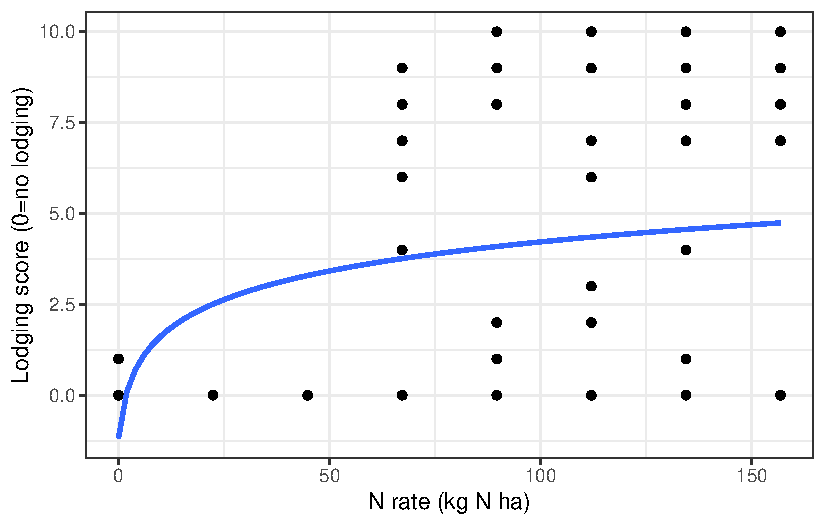
\includegraphics{nrate_draft_files/figure-pdf/unnamed-chunk-4-1.pdf}

We observe a general increase in lodging as nitrogen rate increases. We
fit a logistic curve since lodging cannot be greater than 10 and we
expect as we increase N rate more lodging will get closer to 10. This
curve is obviously not perfect.

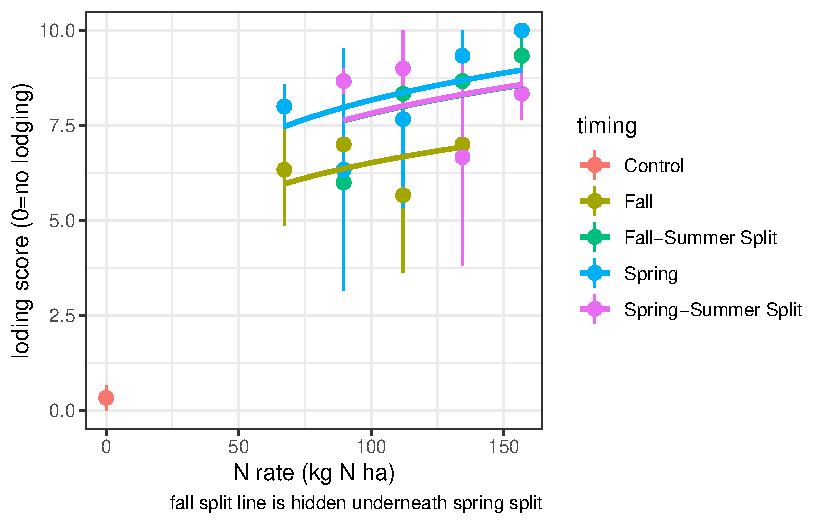
\includegraphics{nrate_draft_files/figure-pdf/unnamed-chunk-6-1.pdf}

Here we are fitting a logistic regression with a y intercept of zero
because we assume at 0N there is no lodging (as shown with control
plots) and that lodging score will increase as nitrogen rate increases
but that lodging will never exceed 10. The takeaway from this figure is
that there is no lodging at 0N and that you see less lodging when you
apply in fall and more when you apply in spring and summer.

\hypertarget{analysis}{%
\subsubsection{Analysis}\label{analysis}}

\begin{verbatim}
Analysis of Variance Table

Response: lodging
                        Df  Sum Sq Mean Sq  F value Pr(>F)    
log(n.total + 1)         1 3109.08 3109.08 428.8900 <2e-16 ***
timing                   5   19.87    3.97   0.5481 0.7388    
log(n.total + 1):timing  3   18.84    6.28   0.8664 0.4655    
Residuals               45  326.21    7.25                    
---
Signif. codes:  0 '***' 0.001 '**' 0.01 '*' 0.05 '.' 0.1 ' ' 1
\end{verbatim}

We reject Ho that the rate of nitrogen does not impact lodging.

We fail to reject Ho that timing has an impact on lodging.

\hypertarget{plant-height}{%
\section{Plant height}\label{plant-height}}

Plant height is also not a measurement of primary interest.

To what extent does plant height relate to lodging in R100?

\hypertarget{r100-year-3}{%
\subsection{R100 year 3}\label{r100-year-3}}

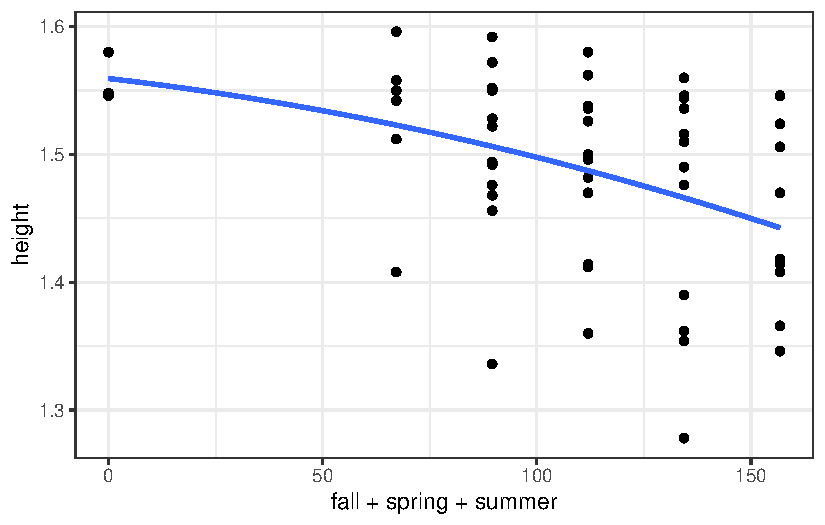
\includegraphics{nrate_draft_files/figure-pdf/unnamed-chunk-8-1.pdf}

We observe an overall trend of decreasing plant height as N rate
increases, modeled best quadratically.

\begin{verbatim}
Analysis of Variance Table

Response: height
                 Df   Sum Sq   Mean Sq F value   Pr(>F)   
poly(n.total, 2)  2 0.050934 0.0254669  5.4217 0.007609 **
timing            4 0.035753 0.0089383  1.9029 0.125627   
Residuals        47 0.220770 0.0046972                    
---
Signif. codes:  0 '***' 0.001 '**' 0.01 '*' 0.05 '.' 0.1 ' ' 1
\end{verbatim}

We reject Ho that nrate does not impact height

We fail to reject Ho that timing has no effect on plant height

We have learned from R100 in it's third stand age that as nrate
increases, there is an increase in lodging and a decrease in plant
height. To what extent are they correlated?

\begin{verbatim}
           lodging     height
lodging  1.0000000 -0.4993655
height  -0.4993655  1.0000000
\end{verbatim}

We observe a pearson correlation coefficient of -0.5 between height and
lodging. This is considered between a moderate and strong correlation.

\hypertarget{yield}{%
\section{Yield}\label{yield}}

\hypertarget{cumulative}{%
\subsection{Cumulative}\label{cumulative}}

Cumulative yield of kernza stands after 3 years of N fertilizer. We are
subsetting dataset, Only V17 and Staples meet this criteria (6 site
years). We sum across stand.age to create a cumulative yield and a
cumulative amount of N applied, then divide both values by 3 to get a
yearly yield\textasciitilde N response.

\hypertarget{quadratic-linear-model-yield-response-to-n}{%
\subsubsection{Quadratic linear model, yield response to
N}\label{quadratic-linear-model-yield-response-to-n}}

\begin{verbatim}
[1] 1020.782
\end{verbatim}

\begin{verbatim}
[1] 1000.713
\end{verbatim}

\begin{verbatim}
Analysis of Variance Table

Response: yield.cum
              Df  Sum Sq Mean Sq F value    Pr(>F)    
poly(cumn, 2)  2 2696949 1348475  12.438 2.607e-05 ***
Residuals     66 7155387  108415                      
---
Signif. codes:  0 '***' 0.001 '**' 0.01 '*' 0.05 '.' 0.1 ' ' 1
\end{verbatim}

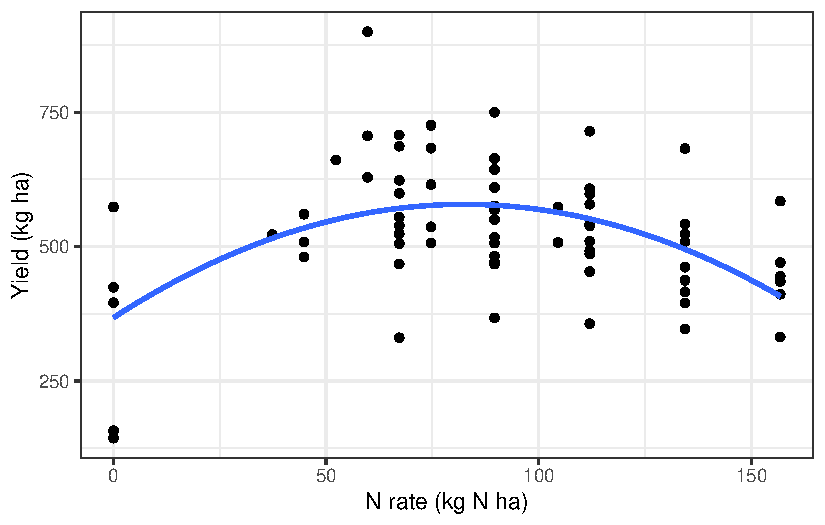
\includegraphics{nrate_draft_files/figure-pdf/unnamed-chunk-12-1.pdf}

We reject the Ho that N rate does not impact yield

Quadratic model provides the best fit

\begin{verbatim}
Analysis of Variance Table

Response: yield.cum
                       Df  Sum Sq Mean Sq F value    Pr(>F)    
poly(cumn, 2)           2 2011131 1005565 12.0239 0.0001701 ***
location                1 2181936 2181936 26.0901 2.065e-05 ***
timing                  2  284394  142197  1.7003 0.2009473    
poly(cumn, 2):location  2  114253   57126  0.6831 0.5132778    
poly(cumn, 2):timing    3  186149   62050  0.7419 0.5360498    
location:timing         2   71804   35902  0.4293 0.6551831    
Residuals              28 2341662   83631                      
---
Signif. codes:  0 '***' 0.001 '**' 0.01 '*' 0.05 '.' 0.1 ' ' 1
\end{verbatim}

We reject Ho that N rate and location do not impact yield

We fail to reject the Ho that timing does not impact yield

\hypertarget{quadratic-linear-mixed-effect-model}{%
\subsubsection{Quadratic linear mixed effect
model}\label{quadratic-linear-mixed-effect-model}}

Here we have our fixed effect of cumulative N, timing and a random
effect of block. Since we only have two sites, location is treated as a
fixed effect.

\begin{verbatim}
Analysis of Deviance Table (Type II Wald chisquare tests)

Response: yield.cum
                                Chisq Df Pr(>Chisq)    
poly(cumn, 2)                  0.5868  2     0.7457    
timing                         4.0312  2     0.1332    
location                      27.2054  1  1.829e-07 ***
poly(cumn, 2):timing           2.8742  3     0.4114    
poly(cumn, 2):location         1.1353  2     0.5669    
timing:location                0.8907  2     0.6406    
poly(cumn, 2):timing:location          0               
---
Signif. codes:  0 '***' 0.001 '**' 0.01 '*' 0.05 '.' 0.1 ' ' 1
\end{verbatim}

We fail to reject Ho that yield does not differ N rate or timing

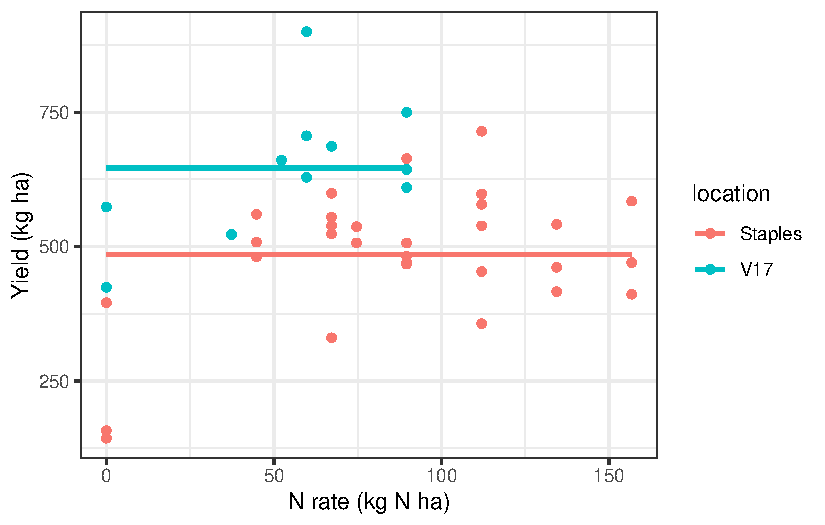
\includegraphics{nrate_draft_files/figure-pdf/unnamed-chunk-15-1.pdf}

TAKEAWAY: We applied N at differing rates and timings over 3 years at
two locations. We cannot reject the Ho that the amount of N and the
timing of N do not impact the cumulative yield over the 3 years when
modelled as a fixed effect model. Personally, I would say our data
suggests at around 60 kg N ha per year results in best grain yields and
then adding more N has no effect. When modeled as a simple quadratic
linear model, we can make this conclusion, but when modelled as a mixed
effect model we cannot.

\hypertarget{yearly-performance}{%
\subsection{Yearly performance}\label{yearly-performance}}

We are using all site years except third stand age of R100 due to high
lodging.

How does N timing and N amount correlate with yield in a given year?

\hypertarget{full-model-site-years-as-random}{%
\subsubsection{Full model, site-years as
random}\label{full-model-site-years-as-random}}

We reject Ho that stand.age, timing and nitrogen rate do not impact
yield

Here we have subsetted data so we have removed instances where a timing
was Fall but no fall N was applied. We only start doing this here
because this is the first time we are looking at timing across years at
each year.

\hypertarget{nitrogen-rate-on-yield}{%
\paragraph{Nitrogen rate on yield}\label{nitrogen-rate-on-yield}}

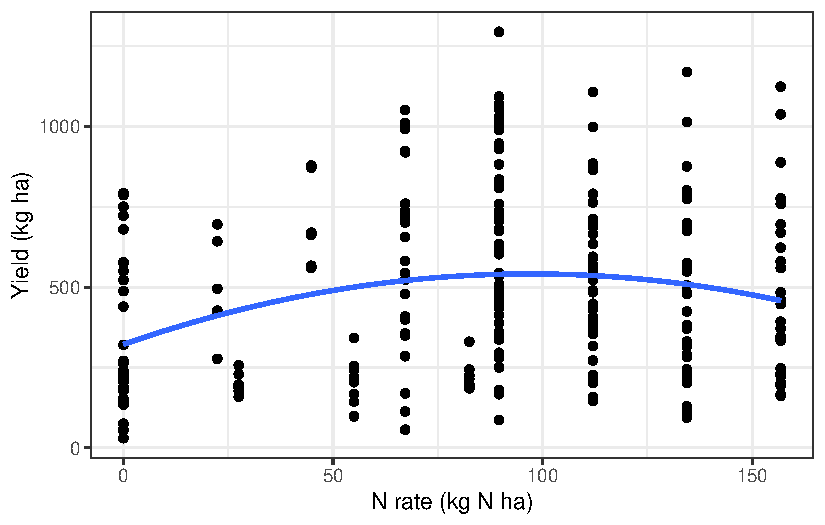
\includegraphics{nrate_draft_files/figure-pdf/nrate effect-1.pdf}

We previously learned the relationship between N rate and yield is best
modelled quadratically and then we rejected Ho that nitrogen rate does
not impact yield. Here we are visualizing the subsetted data used in the
model.

\hypertarget{timing-on-yield}{%
\paragraph{Timing on yield}\label{timing-on-yield}}

\begin{longtable}[]{@{}lllr@{}}
\caption{Estimated marginal means across N rate timings from a mixed
effect model of yield as a function of nitrogen rate, timing and
stand.age across 9 site-years. No interactions were detected among
nitrogen rate, timing and stand age, but main effects were detected from
timing}\tabularnewline
\toprule()
timing & emmean & CI & n \\
\midrule()
\endfirsthead
\toprule()
timing & emmean & CI & n \\
\midrule()
\endhead
Fall & 610 a & 246-975 & 32 \\
Control & 570 ab & 229-912 & 32 \\
Fall-Spring Split & 507 ab & 156-858 & 12 \\
Fall-Summer Split & 505 b & 141-870 & 48 \\
Spring & 456 b & 83-828 & 96 \\
Spring-Summer Split & 420 b & 54-785 & 48 \\
\bottomrule()
\end{longtable}

We reject the Ho that yields were the same regardless of timing.
Applying in the fall was estimated to have a higher grain yield than
when split in the spring, summer or applied alone in the spring.

Since the dataset is unbalanced, we reported estimated marginal means,
95\% confidence intervals and the number of data points within each
timing used in the model.

\hypertarget{full-model-location-as-fixed-effect}{%
\subsubsection{Full model, location as fixed
effect}\label{full-model-location-as-fixed-effect}}

We have 4 locations and there is a rationale to model them as fixed
effects. This puts a lot of stress on our model by cutting it up by n
rate, timing, stand age and location. We end up making a lot of
meaningless comparisons and need to reduce the comparisons we make in
order to prevent a rank deficient model.

We ran a full factorial model, then would remove interaction terms that
were insignificant and rerun the model.

we removed R100 from the dataset (site years = 8) because it only had
one stand age after we removed third stand age for lodging and when
stand.age is modelled as a fixed effect the R100 data doesn't provide
any utility to testing those hypotheses

\begin{verbatim}
Analysis of Deviance Table (Type II Wald chisquare tests)

Response: yield
                                              Chisq Df Pr(>Chisq)    
poly(n.total, 2)                            10.7538  2   0.004622 ** 
timing                                      36.3076  5  8.243e-07 ***
stand.age                                  425.5273  2  < 2.2e-16 ***
location                                   156.3313  2  < 2.2e-16 ***
poly(n.total, 2):timing                      4.0963  7   0.768623    
poly(n.total, 2):stand.age                   7.5965  4   0.107527    
timing:stand.age                            14.8525  8   0.062079 .  
poly(n.total, 2):location                    2.2606  3   0.520119    
timing:location                              2.4905  2   0.287867    
stand.age:location                          39.9292  3  1.103e-08 ***
poly(n.total, 2):timing:stand.age            2.1166 10   0.995366    
poly(n.total, 2):timing:location                     0               
poly(n.total, 2):stand.age:location          2.0729  4   0.722358    
timing:stand.age:location                    0.3926  2   0.821752    
poly(n.total, 2):timing:stand.age:location           0               
---
Signif. codes:  0 '***' 0.001 '**' 0.01 '*' 0.05 '.' 0.1 ' ' 1
\end{verbatim}

\begin{verbatim}
Analysis of Deviance Table (Type II Wald chisquare tests)

Response: yield
                     Chisq Df Pr(>Chisq)    
poly(n.total, 2)    17.991  2   0.000124 ***
timing              32.370  5  5.018e-06 ***
stand.age          390.718  2  < 2.2e-16 ***
location           163.091  2  < 2.2e-16 ***
stand.age:location  76.858  3  < 2.2e-16 ***
---
Signif. codes:  0 '***' 0.001 '**' 0.01 '*' 0.05 '.' 0.1 ' ' 1
\end{verbatim}

Change in yield over stand.age was different, Staples when down in year
2 and V17 went up. We will need to separate by location or stand age.

\hypertarget{slice-by-stand-age}{%
\paragraph{Slice by stand age}\label{slice-by-stand-age}}

It would be interesting to know if there is an ideal N rate or timing in
year 1 and then a different one in year 2 or year 3, but Ho could not be
rejected in year 1 and there were location*timing interactions in year
3.

Slicing by second stand age yielded the only interesting results.

\begin{verbatim}
Analysis of Deviance Table (Type II Wald chisquare tests)

Response: yield
                                    Chisq Df Pr(>Chisq)    
poly(n.total, 2)                  14.3748  2   0.000756 ***
timing                            30.0587  5  1.436e-05 ***
location                         118.6736  2  < 2.2e-16 ***
poly(n.total, 2):timing            4.1718  6   0.653435    
poly(n.total, 2):location          2.9520  3   0.399092    
timing:location                    0.5350  2   0.765288    
poly(n.total, 2):timing:location           0               
---
Signif. codes:  0 '***' 0.001 '**' 0.01 '*' 0.05 '.' 0.1 ' ' 1
\end{verbatim}

\begin{longtable}[]{@{}lllr@{}}
\caption{Estimated marginal means across N rate timings from a mixed
effect model of yield in second year kernza stands as a function of
nitrogen rate, timing and location. No interactions were detected among
nitrogen rate, timing and location, but main effects were detected from
timing}\tabularnewline
\toprule()
timing & emmean & CI & n \\
\midrule()
\endfirsthead
\toprule()
timing & emmean & CI & n \\
\midrule()
\endhead
Fall & 768 a & 677-860 & 16 \\
Fall-Summer Split & 722 ab & 615-829 & 12 \\
Fall-Spring Split & 670 abc & 518-821 & 4 \\
Control & 638 abc & 346-929 & 11 \\
Spring & 585 bc & 503-667 & 31 \\
Spring-Summer Split & 520 c & 413-627 & 12 \\
\bottomrule()
\end{longtable}

TAKEAWAY: across 8 site-years, second year yields were higher when N was
applied in the fall versus in the spring or a spring summer split. They
were also higher in the Fall summer split compared with the spring
summer split

\hypertarget{slice-by-site}{%
\paragraph{slice by site}\label{slice-by-site}}

Lastly, we can slice by site and do an independent analysis for each
site. This is what Dominic did and I did in my exploratory data
analysis.

The main takeaway is we see a great response from staples but not much
beyond that site.

R100 had lodging and is weird because treatments were started till year
2. V17 was kinda limited in a good range of nitrogen rates and NDSU
didn't show much response because it was hot and dry when they put down
their urea and they only did a spring timing. The messyness of these
sites may be better shown in the combined analysis of all site years.

\hypertarget{staples-1}{%
\subparagraph{Staples}\label{staples-1}}

\begin{verbatim}
Analysis of Deviance Table (Type II Wald chisquare tests)

Response: yield
                                     Chisq Df Pr(>Chisq)    
poly(n.total, 2)                   11.1970  2   0.003703 ** 
stand.age                         317.2548  2  < 2.2e-16 ***
timing                             33.8945  4  7.833e-07 ***
poly(n.total, 2):stand.age          6.8114  4   0.146200    
poly(n.total, 2):timing             3.6056  6   0.729878    
stand.age:timing                   12.9043  7   0.074475 .  
poly(n.total, 2):stand.age:timing   1.9117 10   0.996973    
---
Signif. codes:  0 '***' 0.001 '**' 0.01 '*' 0.05 '.' 0.1 ' ' 1
\end{verbatim}

Beautiful main effects and no interactions

\begin{longtable}[]{@{}lrl@{}}
\toprule()
stand.age & observed\_mean & tukey \\
\midrule()
\endhead
1 & 754.4952 & a \\
2 & 528.7498 & b \\
3 & 257.7972 & c \\
\bottomrule()
\end{longtable}

\begin{longtable}[]{@{}lrl@{}}
\toprule()
timing & observed\_mean & tukey \\
\midrule()
\endhead
Fall & 541.0500 & a \\
Fall-Summer Split & 535.4278 & ab \\
Spring & 513.0013 & abc \\
Spring-Summer Split & 464.6167 & bc \\
Control & 232.2756 & c \\
\bottomrule()
\end{longtable}

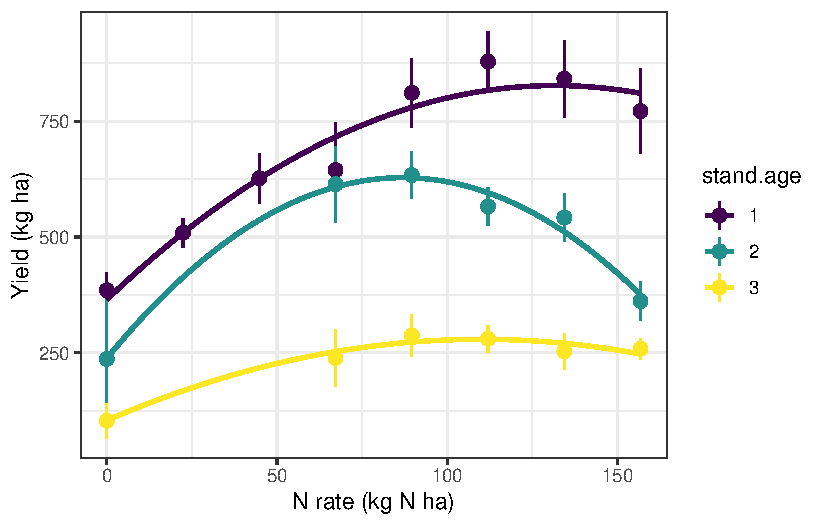
\includegraphics{nrate_draft_files/figure-pdf/nrate-1.pdf}

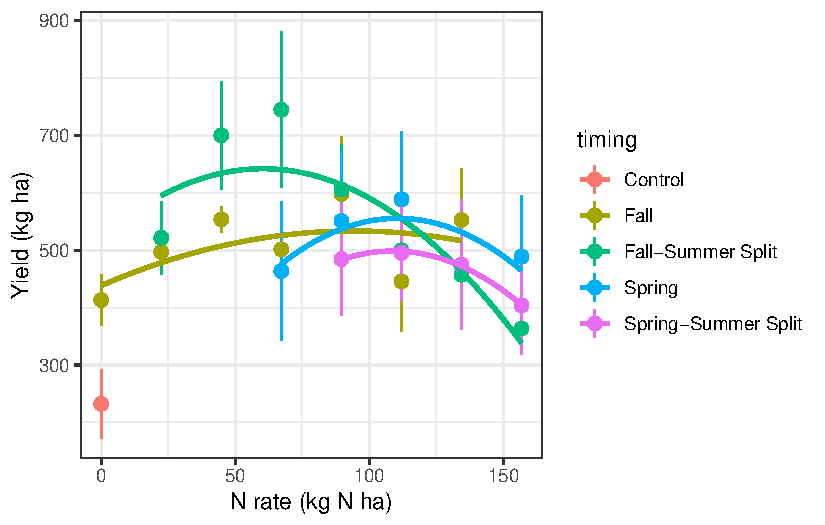
\includegraphics{nrate_draft_files/figure-pdf/unnamed-chunk-21-1.pdf}

A lot of interesting interpretations here and options for extrapolation

\hypertarget{refs}{}
\begin{CSLReferences}{1}{0}
\leavevmode\vadjust pre{\hypertarget{ref-lme4}{}}%
Bates, Douglas, Martin Mächler, Ben Bolker, and Steve Walker. 2015.
{``Fitting {Linear} {Mixed}-{Effects} {Models} {Using} Lme4.''}
\emph{Journal of Statistical Software} 67 (1): 1--48.
\url{https://doi.org/10.18637/jss.v067.i01}.

\leavevmode\vadjust pre{\hypertarget{ref-car}{}}%
Fox, John, and Sanford Weisberg. 2019. \emph{An {R} {Companion} to
{Applied} {Regression}}. Third. Thousand Oaks CA: Sage.
\url{https://socialsciences.mcmaster.ca/jfox/Books/Companion/}.

\leavevmode\vadjust pre{\hypertarget{ref-multcomp}{}}%
Hothorn, Torsten, Frank Bretz, and Peter Westfall. 2008. {``Simultaneous
{Inference} in {General} {Parametric} {Models}.''} \emph{Biometrical
Journal} 50 (3): 346--63.

\leavevmode\vadjust pre{\hypertarget{ref-emmeans}{}}%
Lenth, Russell V. 2022. \emph{Emmeans: {Estimated} {Marginal} {Means},
Aka {Least}-{Squares} {Means}}.
\url{https://CRAN.R-project.org/package=emmeans}.

\leavevmode\vadjust pre{\hypertarget{ref-R}{}}%
R Core Team. 2022. \emph{R: A Language and Environment for Statistical
Computing}. Vienna, Austria: R Foundation for Statistical Computing.
\url{https://www.R-project.org/}.

\leavevmode\vadjust pre{\hypertarget{ref-tidyverse}{}}%
Wickham, Hadley, Mara Averick, Jennifer Bryan, Winston Chang, Lucy
D'Agostino McGowan, Romain François, Garrett Grolemund, et al. 2019.
{``Welcome to the Tidyverse.''} \emph{Journal of Open Source Software} 4
(43): 1686. \url{https://doi.org/10.21105/joss.01686}.

\end{CSLReferences}



\end{document}
